%%%%%%%%%%%%%%%%%%%%%%%%%%%%%%%%%%%%%%%%%%%%%%%%%%%%%%%%
%%%%%%%%%%%%%%%%%%%%%%%%%%%%%%%%%%%%%%%%%%%%%%%%%%%%%%%%
%%%%%%%%%%%%%%%%%%%%%%%%%%%%%%%%%%%%%%%%%%%%%%%%%%%%%%%%
\chapter{Supervised Learning}
\label{ml:supervised}

In supervised learning a model is trained over many known examples
to use input features $\mathbf{X}$ to make a prediction \yhat about the true value $y$.
During the training process parameters $\beta$ of
the model are adjusted to minimize a two-part objective function,
$S\left(\beta\right) = L\left(\beta\right) + \Omega\left(\beta\right)$.
The training loss $L\left(\beta\right)$ measures the model's predictive performance
while $\Omega\left(\beta\right)$ is a regularization term to penalize model complexity.
Note that $L$ is a measure of the model's bias,
while $\Omega$ is --- somewhat --- a measure of its variance,
so $S\left(\beta\right)$ captures both parts of the bias-variance tradeoff \cite{HastieTF09}.

%%%%%%%%%%%%%%%%%%%%%%%%%%%%%%%%%%%%%%%%%%%%%%%%%%%%%%%%
%%%%%%%%%%%%%%%%%%%%%%%%%%%%%%%%%%%%%%%%%%%%%%%%%%%%%%%%
\section{(Gaussian) N{a\"i}ve Bayes Classification (GNB)}
\label{ml:supervised:Bayes}
% TODO
% TODO maximum a posteriori (italics) probability (MAP) estimator

%%%%%%%%%%%%%%%%%%%%%%%%%%%%%%%%%%%%%%%%%%%%%%%%%%%%%%%%
%%%%%%%%%%%%%%%%%%%%%%%%%%%%%%%%%%%%%%%%%%%%%%%%%%%%%%%%
\section{\texorpdfstring{$k$}{k}-Nearest Neighbors (\texorpdfstring{$k$}{k}-NN)}
\label{ml:supervised:kNN}
% TODO
% TODO also talk about collaborative filtering

%%%%%%%%%%%%%%%%%%%%%%%%%%%%%%%%%%%%%%%%%%%%%%%%%%%%%%%%
%%%%%%%%%%%%%%%%%%%%%%%%%%%%%%%%%%%%%%%%%%%%%%%%%%%%%%%%
\section{Support Vector Machines (SVM)}
\label{ml:supervised:SVM}

Basic support vector machines (SVM) work by finding a hyperplane in the $n$-dimensional
feature space of the training data which best separate the different classes.
This is done by maximizing the margin, $2/\norm{\mathbf{w}}$,
around the hyperplane defined by $\innerproduct{\mathbf{w}}{\mathbf{x}} - b = 0$,
where $\innerproduct{\mathbf{a}}{\mathbf{b}}$ is the inner product.
For the separable case, as shown in \cref{fig:svm_sep}, this
can be done by minimizing $\norm{\mathbf{w}}$, with the hard-margin condition that
$y_{i} \left(\innerproduct{\mathbf{w}}{\mathbf{x}_{i}} - b\right)$ for all $1 \leq i \leq m$.

However, in reality the data are frequently inseparable and we must switch
to a soft-margin objective function \cref{eq:svm:soft_margin_obj}.
A hinge loss function is included to penalize points on the ``wrong'' side of the margin
proportionally to their distance from the margin.
Here the $\lambda$ hyperparameter sets the tradeoff between
margin size and ensuring points land on their correct sides.

\begin{equation} \label{eq:svm:soft_margin_obj}
S\left(\mathbf{w}, b\right) =
\lambda\, \norm{\mathbf{w}}^{2}
+ \frac{1}{m} \sum_{i=1}^{m} \,
\max{\big(0,\, 1 - y_{i} \left(\innerproduct{\mathbf{w}}{\mathbf{x}_{i}} - b\right)\big)}.
\end{equation}

\begin{figure}[H]
\centering
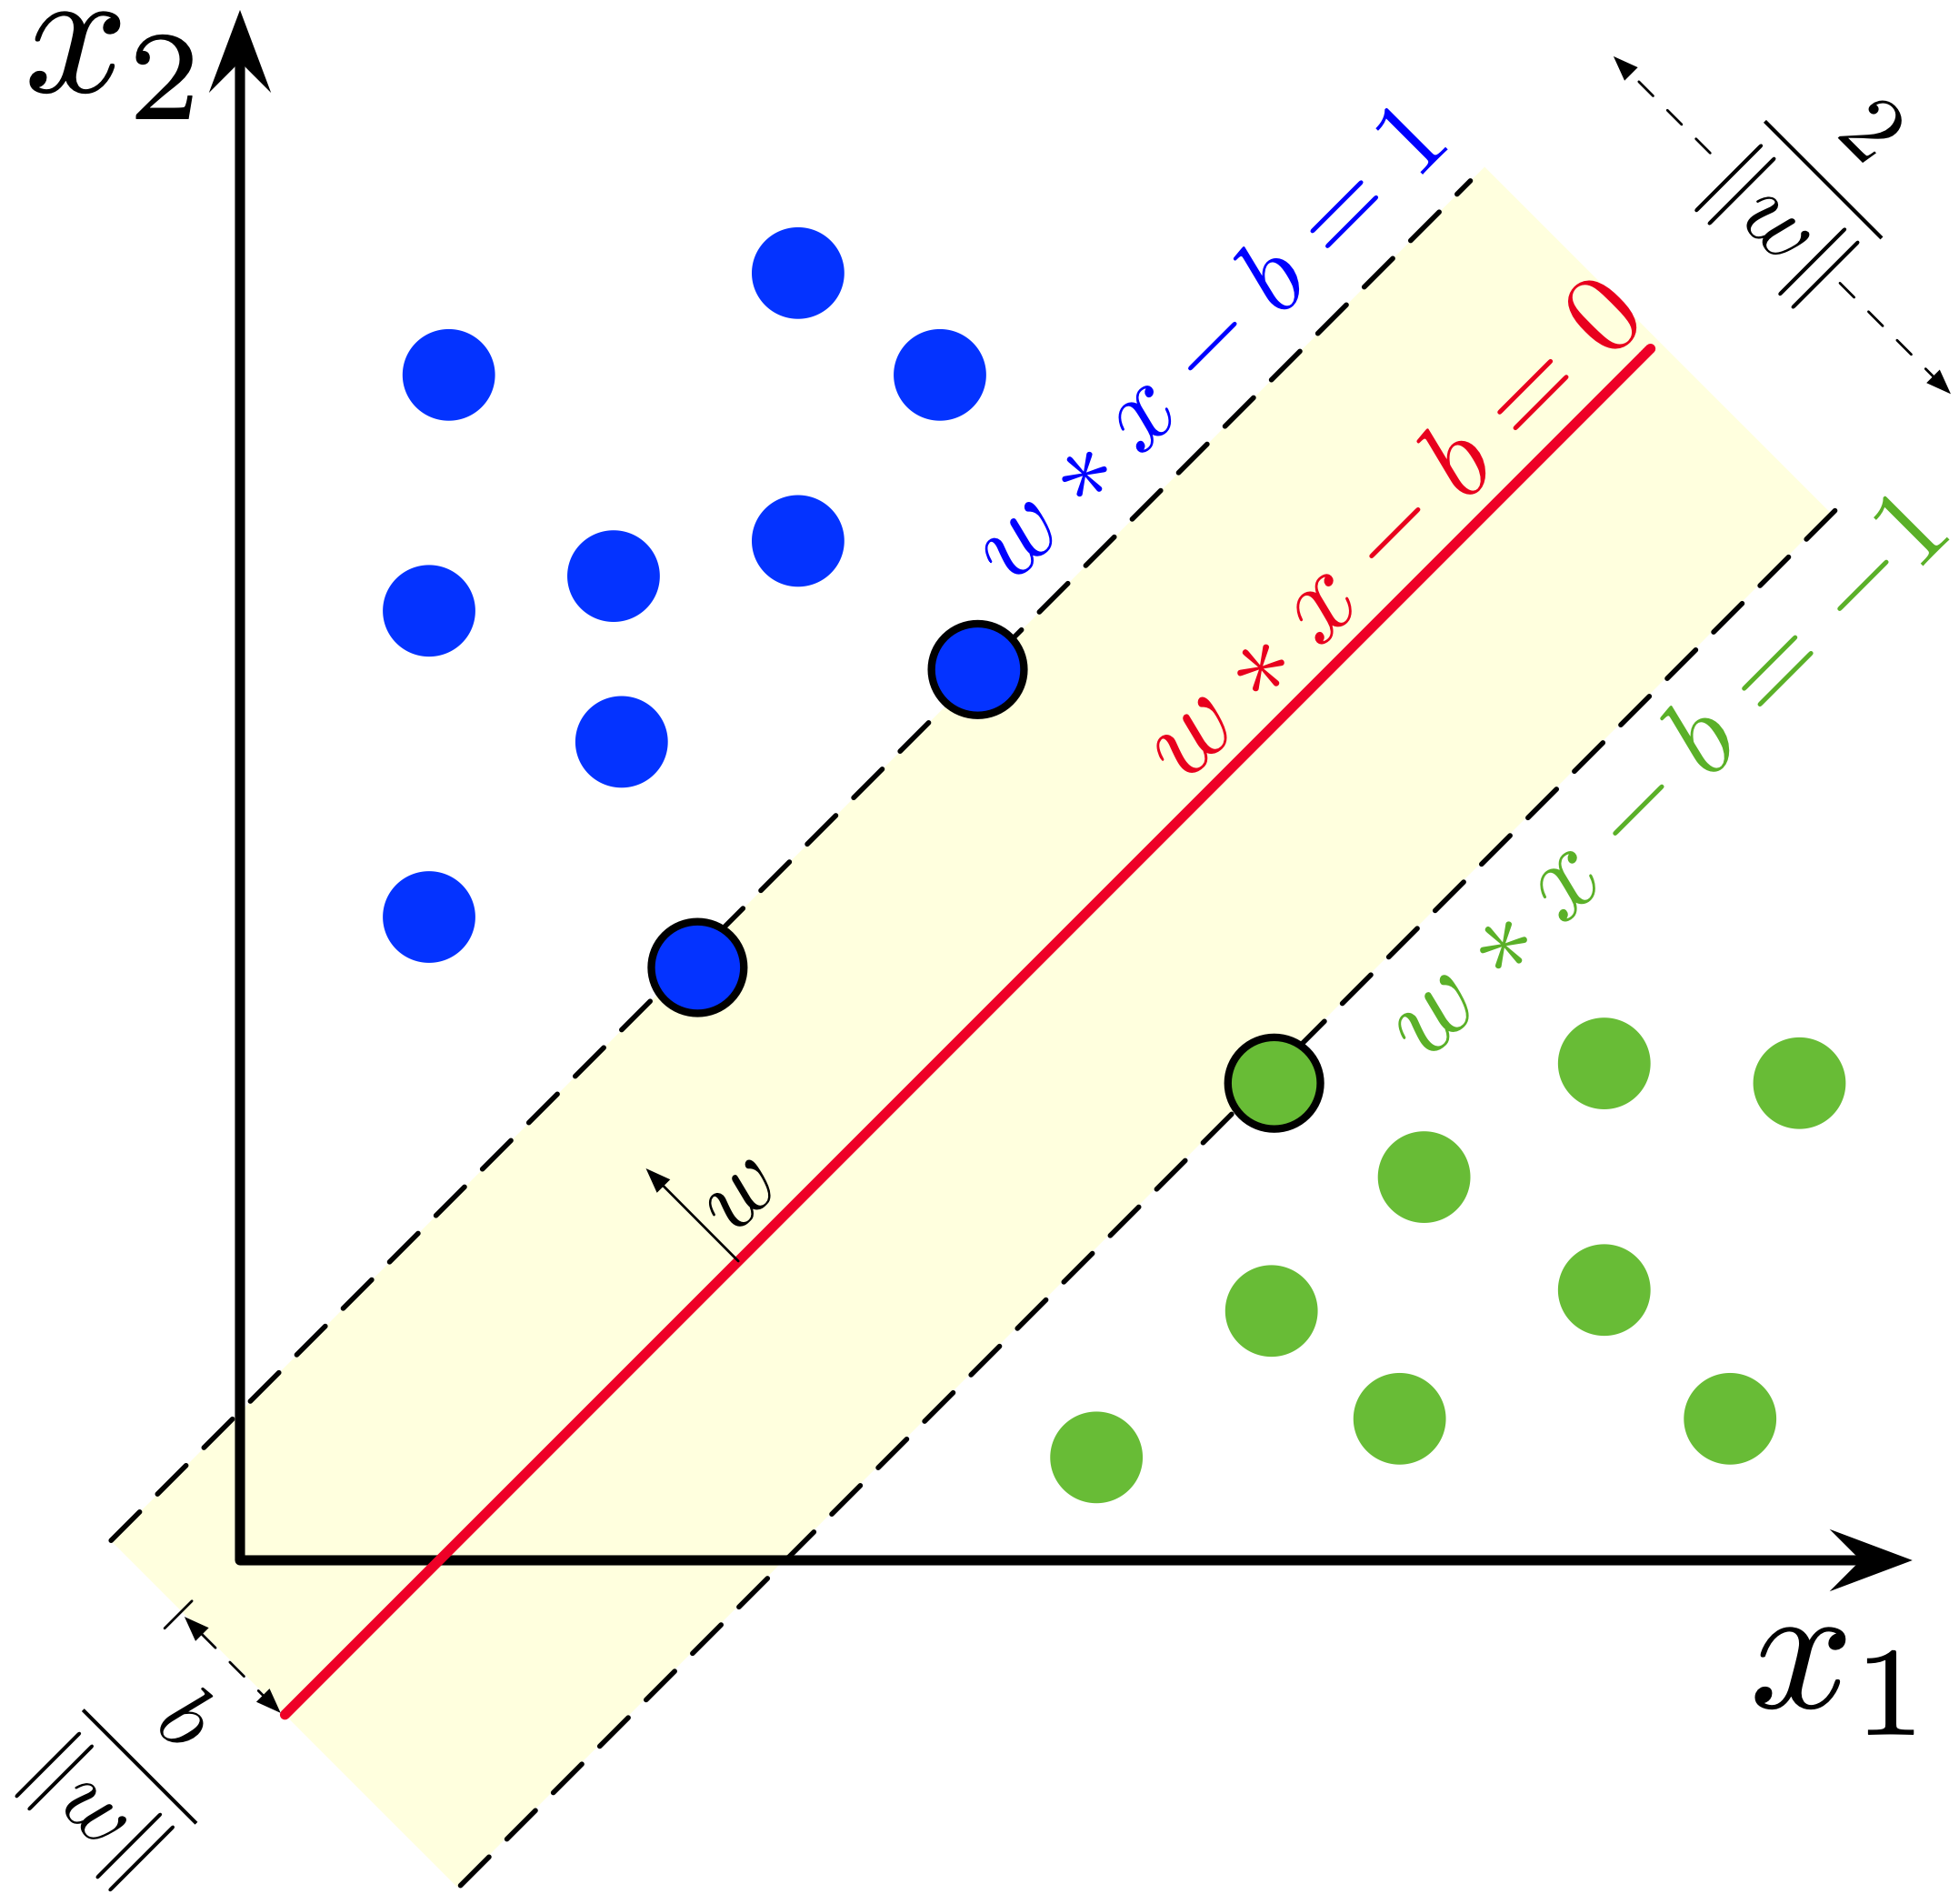
\includegraphics[width=0.42\textwidth]{figures/ml/svm_margin.png}
\vspace{0.2cm}
\caption{
Illustration of the SVM method in the separable case,
by \href{https://en.wikipedia.org/wiki/File:SVM_margin.png}{Larhmam}.
The trained hyperplane in red separates the two classes by the largest margin.
The data points on the margin boundary with black boarders
are known as support vectors, since out of all the data
they are the points really fixing the hyperplane and margin.
}
\label{fig:svm_sep}
\end{figure}

To gain better performance still, we can recast the problem in
a new higher dimensional space where the classes may be easier to separate with a hyperplane.
Fortunately, we don't even need to fully specify the new space,
just a non-linear kernel function\footnote{Common kernel choices include
polynomials of the inner product,
the Gaussian radial basis function,
and the hyperbolic tangent.} $k\left(\mathbf{a},\mathbf{b}\right)$
in place of the standard inner product. This is known as the kernel trick.
The classification boundary in the original feature space can then become non-linear,
as can be seen in \cref{fig:svm_kernel_trick}.

\vspace{-0.3cm}% TODo hard coded to fit on one page

\begin{figure}[H]
\centering
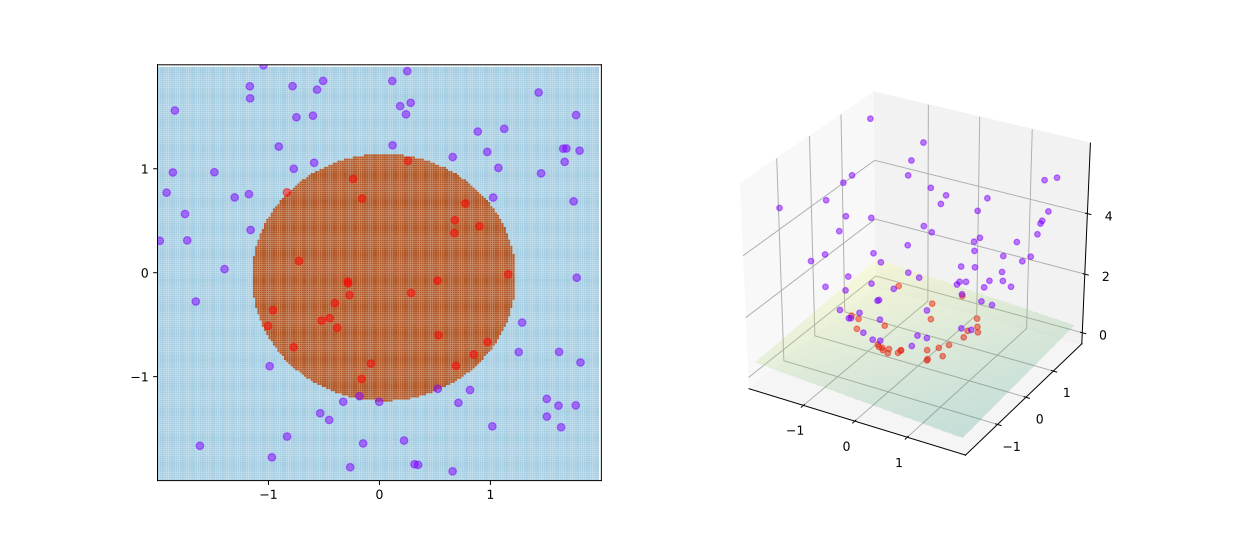
\includegraphics[width=0.8\textwidth,trim={4.0cm 0.8cm 4.0cm 1.4cm},clip]{figures/ml/kernel_trick_example.png}% trim={<left> <lower> <right> <upper>}
\caption{
Graphical example of the kernel trick, by \href{https://en.wikipedia.org/wiki/File:Kernel_trick_idea.svg}{Shiyu Ji}.
Here the kernel $k\left(\mathbf{a},\mathbf{b}\right) = \innerproduct{\mathbf{a}}{\mathbf{b}} + \norm{\mathbf{a}}^{2} \norm{\mathbf{b}}^{2}$
transforms the red and purple classes, linearly inseparable in $n=2$ dimensions on the left,
to a separable $3$-dimensional space on the right.
}
\label{fig:svm_kernel_trick}
\end{figure}

In practice minimizing $S\left(\mathbf{w}, b\right)$ can be
performed more readily by instead solving the Lagrangian dual problem,
which is computationally efficient to solve with quadratic programming algorithms.
Other modern techniques developed to tackle large and sparse data include
sub-gradient methods and coordinate descent\footnote{Sub-gradient methods work better for large $m$,
coordinate descent for large $n$.}.
However, compared to other classifiers SVM training times
tend to slow significantly for large datasets,
in \sklearn\footnote{See the
\href{https://scikit-learn.org/stable/modules/generated/sklearn.svm.SVC.html}{documentation}
for \texttt{sklearn.svm.SVC}.
\texttt{LinearSVC} may be faster.
The best performance I've seen quoted is $\order{n m \log{\left(m\right)}}$.} by
at least $\order{m^{2}}$, limiting $m \sim \num{e4}$.

%\begin{figure}[H]
%  \centering
%  \begin{subfigure}[b]{0.48\textwidth}\centering
%      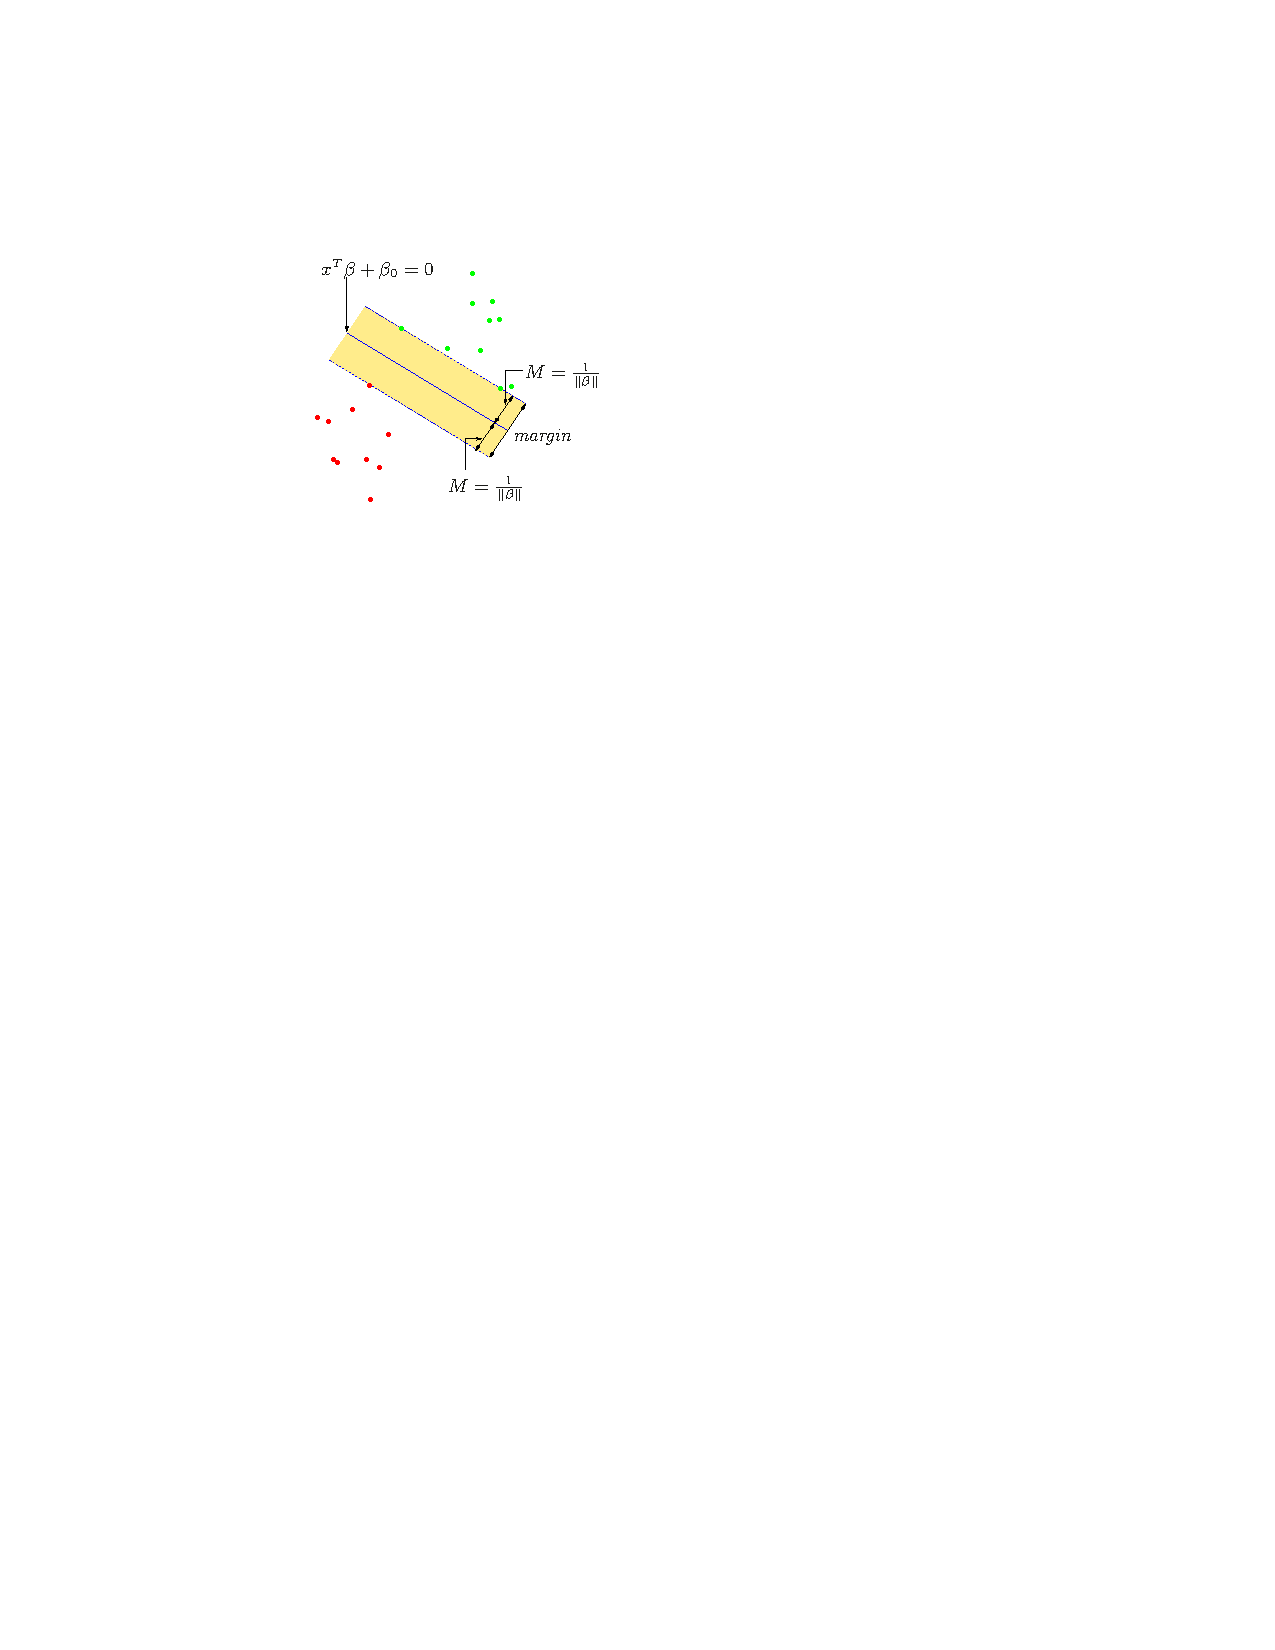
\includegraphics[width=\textwidth]{figures/ml/svm_separable}
%  \caption{Separable}
%  \label{fig:svm:separable}
%  \end{subfigure}
%  ~
%  \begin{subfigure}[b]{0.48\textwidth}\centering
%      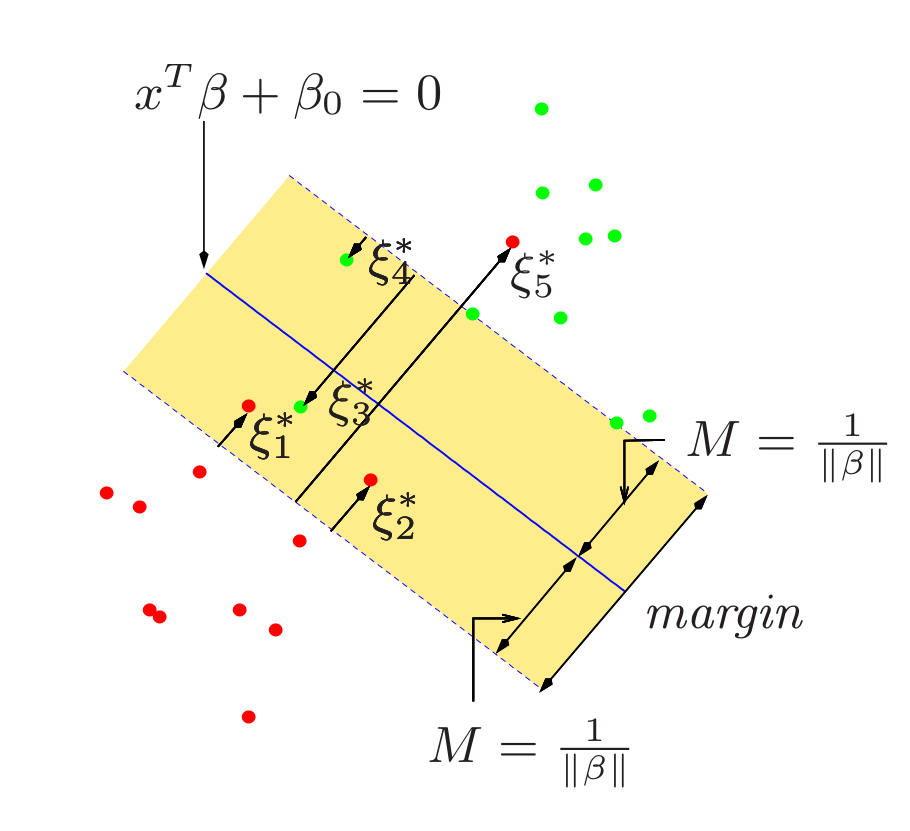
\includegraphics[width=\textwidth]{figures/ml/svm_nonseparable}
%  \caption{Nonseparable}
%  \label{fig:svm:nonseparable}
%  \end{subfigure}
%\caption{
%Illustrations of SVMs in the separable and nonseparable case \cite{HastieTF09}.
%\label{fig:svm}
%}
%\end{figure}

%%%%%%%%%%%%%%%%%%%%%%%%%%%%%%%%%%%%%%%%%%%%%%%%%%%%%%%%
%%%%%%%%%%%%%%%%%%%%%%%%%%%%%%%%%%%%%%%%%%%%%%%%%%%%%%%%
\section{Decision Trees, \texorpdfstring{\ie}{ie} Classification and Regression Trees (CART)}
\label{ml:supervised:CART}

A basic classifier can be created from a tree of selections on $\mathbf{X}$ designed to
separate the classes at each branch.
Such a model is known as a classification and regression tree (CART) \cite{Breiman:2253780}
and a simple example can be found in \cref{ml:supervised:CART:small_example_CART}.
As the splits are just selections on the input variables,
they are --- somewhat --- possible to understand,
and conveniently do not need any kind of feature scaling, unlike other methods.
To make a prediction for an event the tree and its branches are traversed
until the event lands in one of the weighted leaves.
The weight of the leaf $w$ is positive (negative) for signal-like (background-like) events.
A logistic function is used to properly transform $w$ into an output score
$\yhat = 1 /\left(1+e^{-w}\right)$ within $0 < \yhat < 1$.

\begin{figure}[H]
\centering
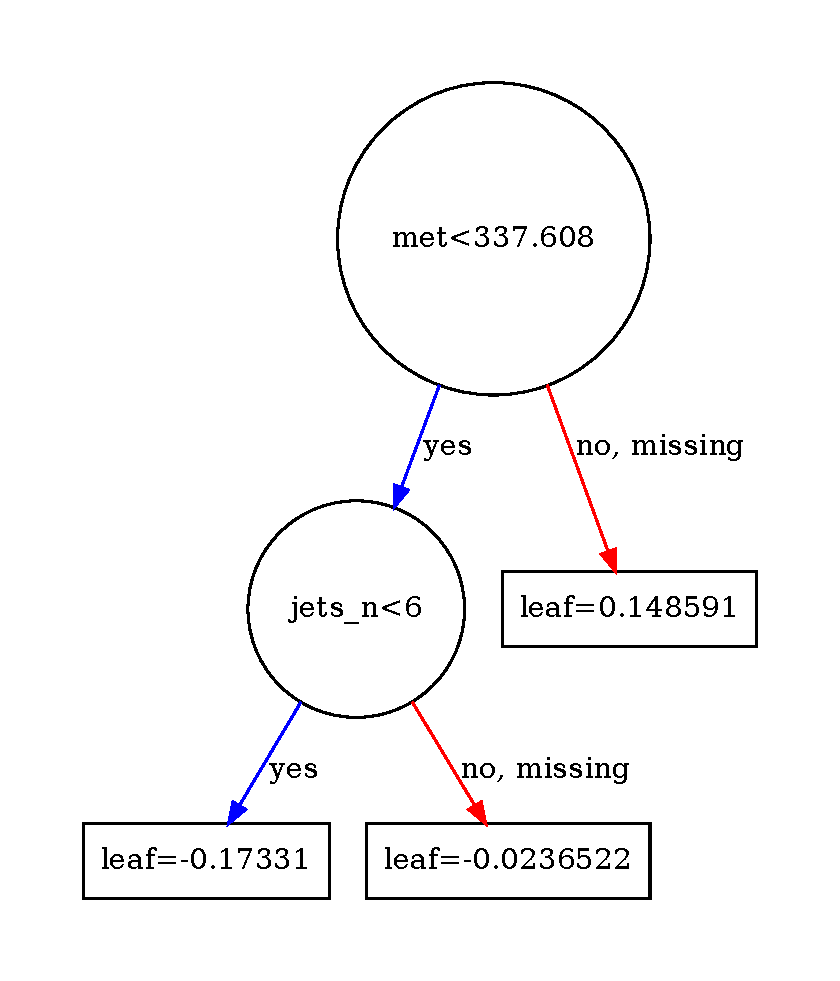
\includegraphics[width=0.4\textwidth]{figures/ml/tree7_g2000_n1200}
\caption{
Simple classification and regression tree (CART).
Signal-like (background-like) events receive positive (negative) weights in the leaves.
}
\label{ml:supervised:CART:small_example_CART}
\end{figure}

% TODO include gini impurity / importance

%%%%%%%%%%%%%%%%%%%%%%%%%%%%%%%%%%%%%%%%%%%%%%%%%%%%%%%%
%%%%%%%%%%%%%%%%%%%%%%%%%%%%%%%%%%%%%%%%%%%%%%%%%%%%%%%%
\section{Boosted Decision Trees (BDT)}
\label{ml:supervised:BDT}

Individual CARTs are rather poor and limited models
in terms of the behaviors they can successfully predict.
However, by taking an ensemble of $K$ complementary trees, \ie boosting \cite{FREUND1997119,friedman2000},
and summing each CART's individual weight $w_{k}$ a much more flexible BDT\footnote{As the leaf weights
are reals rather than integer classes this approach may be better described as a boosted regression tree,
and can indeed handle regression problems without the logistic function.} is formed.
The component trees of a BDT are generated by iteratively adding new trees $f_{k}\left(x_{i}\right)$ to those which came before \cite{XGBoost},

\begin{equation} \label{eq:boosting}
\begin{aligned}
\hat{y}^{\left(0\right)} &= 0\,, \\
\hat{y}^{\left(1\right)} &= f_1\left(\mathbf{X}\right) = \hat{y}^{\left(0\right)} + f_1\left(\mathbf{X}\right), \\
\hat{y}^{\left(2\right)} &= f_1\left(\mathbf{X}\right) + f_2\left(\mathbf{X}\right)= \hat{y}^{\left(1\right)} + f_2\left(\mathbf{X}\right), \\
                           &\vdotswithin{\displaystyle =} \\
\hat{y}^{\left(t\right)} &= \sum_{k=1}^t f_k\left(\mathbf{X}\right)= \hat{y}^{\left(t-1\right)} + f_t\left(\mathbf{X}\right),
\end{aligned}
\end{equation}

\noindent where each tree $f_{k}$ is grown from zero branches while minimizing $S\left(\beta\right)$.
Through the ingenious use of a second order Taylor expansion this process can
be recast as a form of gradient descent, and thus is known as
stochastic gradient boosting \cite{10.2307/2699986,FRIEDMAN2002367}.
The number of boosting rounds, and thus trees, $K$ can be chosen in advance
but is better optimized during the training process via early stopping.

%%%%%%%%%%%%%%%%%%%%%%%%%%%%%%%%%%%%%%%%%%%%%%%%%%%%%%%%
\subsection{\xgboost}% would rather have the \textsc caps than italics
\label{ml:supervised:BDT:xgboost}
% TODO see https://towardsdatascience.com/boosting-algorithm-xgboost-4d9ec0207d
% TODO how does the Hessian come into play

The \xgboost\footnote{\xgboost: eXtreme Gradient Boosting, \href{https://github.com/dmlc/xgboost}{github.com/dmlc/xgboost}.} library \cite{XGBoost}
is a modern open source implementation of gradient boosted decision tree methods.
Through various algorithmic and memory optimizations \xgboost demonstrates good performance\footnote{\xgboost has lost
its lead in recent years to newer libraries such as LightGBM \cite{LightGBM}
and CatBoost \cite{CatBoost}.}.
L1 and L2 regularization is incorporated via

\begin{equation} \label{eq:bdt_omega_reg}
\Omega\left(f\right) = \alpha T + \frac{1}{2}\lambda \sum_{j=1}^T w_j^2\,,
\end{equation}

\noindent where $T$ is the number of leaves in a tree and $w_{j}$ are the leaf weights;
however, the default hyperparameters $\alpha=0$ and $\lambda=1$ only enable L2 regularization.
Other important hyperparameters in \xgboost include the
learning rate $\eta$, which scales the corrections added by each new tree,
maximum tree depth, which sets a limit on the complexity of any tree via its depth,
and the early stopping validation threshold.
For reference $\eta=0.3$ and a maximum depth of 6 are the default values.

%%%%%%%%%%%%%%%%%%%%%%%%%%%%%%%%%%%%%%%%%%%%%%%%%%%%%%%%
\subsection{AdaBoost}
\label{ml:supervised:BDT:AdaBoost}
% TODO

%%%%%%%%%%%%%%%%%%%%%%%%%%%%%%%%%%%%%%%%%%%%%%%%%%%%%%%%
%%%%%%%%%%%%%%%%%%%%%%%%%%%%%%%%%%%%%%%%%%%%%%%%%%%%%%%%
\section{Random Forest}
\label{ml:supervised:RF}
% TODO

% TODO best results occur when you chose $\sqrt{n}$ features randomly to build each tree

%%%%%%%%%%%%%%%%%%%%%%%%%%%%%%%%%%%%%%%%%%%%%%%%%%%%%%%%
%%%%%%%%%%%%%%%%%%%%%%%%%%%%%%%%%%%%%%%%%%%%%%%%%%%%%%%%
\section{Artificial Neural Networks (NN)}
\label{ml:supervised:ANN}
% TODO

% TODO add back prop somewhere, here or in grad descent

\begin{figure}[H]
  \centering
  \begin{subfigure}[b]{0.48\textwidth}\centering
      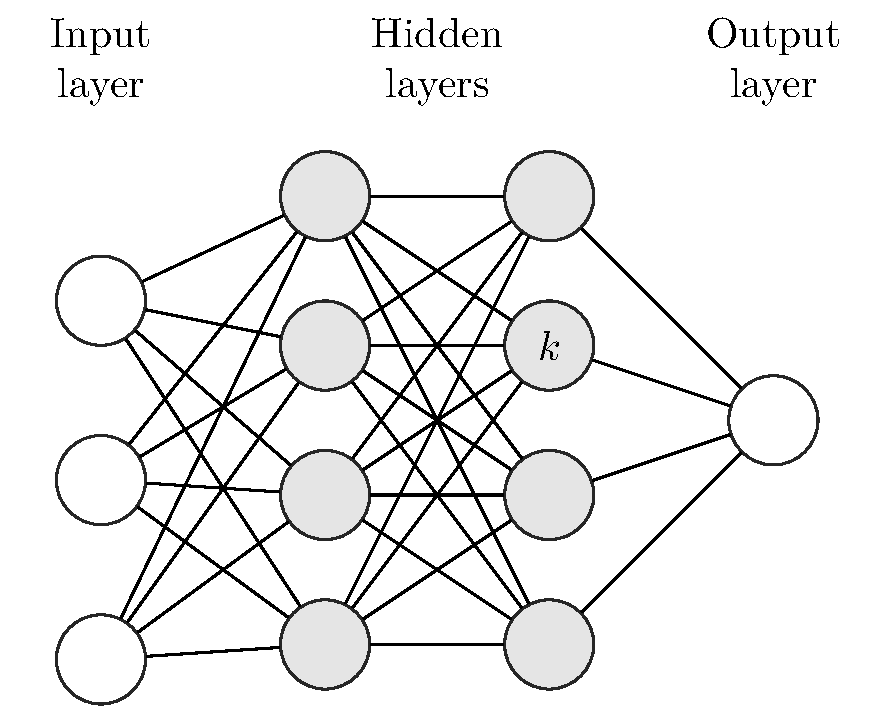
\includegraphics[width=\textwidth]{figures/ml/NN_diagram/NN_diagram}
  \caption{NN Example}
  \label{fig:NN:ex}
  \end{subfigure}
  ~
  \begin{subfigure}[b]{0.48\textwidth}\centering
      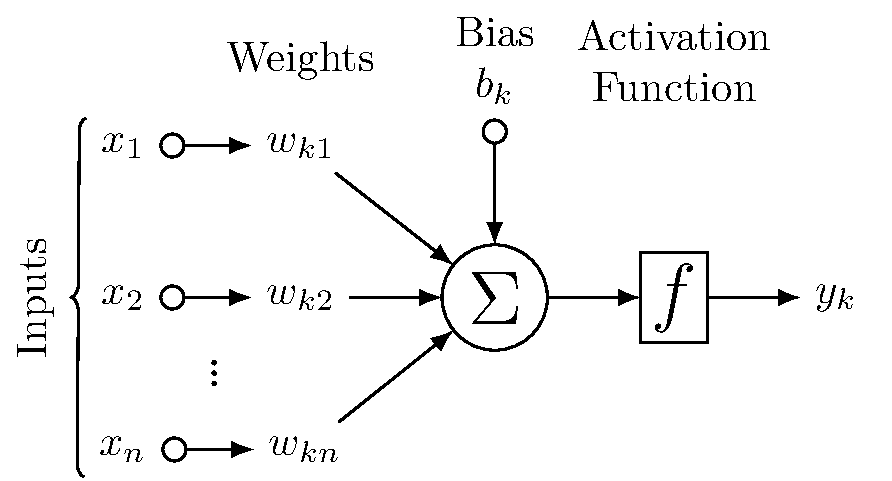
\includegraphics[width=\textwidth]{figures/ml/NN_neuron/NN_neuron}
  \caption{Neuron}
  \label{fig:NN:Neuron}
  \end{subfigure}
\caption{
Illustrations of the components of a neural network.
\label{fig:NN}
}
\end{figure}
